\chapter{Research Design}
    In this chapter we discuss various issues and techniques that should be considered when conducting empirical analyses.

    \section{Controls and Causality}

        In our investigations, we seek to find causality. One way we have found is to introduce controls to avoid omitted variable bias. However adding more covariates is not necessarily better as we will show.

        \subsection{Bad controls}
    
            \begin{example}
                Take for example the experiment:
                \begin{align}
                    (\text{test score})_i = \beta_0 + \beta_1(\text{class size})_i +\beta_c(\text{controls})_i+u_i
                \end{align}
                where:
                \begin{align}
                    (\text{class size})_i = \frac{(\text{students})_i}{(\text{teachers})_i}
                \end{align}
                and
                \begin{align}
                    (\text{total exp./student})_i
                        &= \text{wage}\times \frac{(\text{teachers})_i }{(\text{students})_i}+\frac{(\text{other expenditures})_i }{(\text{students})_i}\\
                        &= \text{wage}\times \frac{1}{(\text{class sizes})_i}+\frac{(\text{other expenditures})_i }{(\text{students})_i}
                \end{align}
                We would like to see the effect of class sizes on test scores. It would seem intuitive to control for total expenditures right? 
                \begin{figure}[h]
                    \centering
                    

\tikzset{every picture/.style={line width=0.75pt}} %set default line width to 0.75pt        

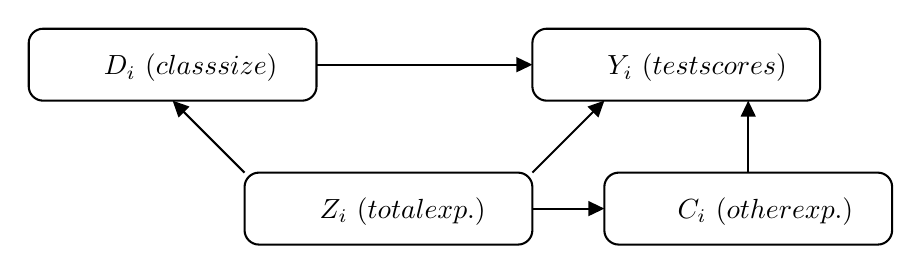
\begin{tikzpicture}[x=0.65pt,y=0.65pt,yscale=-1,xscale=1]
%uncomment if require: \path (0,361); %set diagram left start at 0, and has height of 361

%Straight Lines [id:da16218237230483512] 
\draw    (470,160) -- (470,123) ;
\draw [shift={(470,120)}, rotate = 90] [fill={rgb, 255:red, 0; green, 0; blue, 0 }  ][line width=0.08]  [draw opacity=0] (8.93,-4.29) -- (0,0) -- (8.93,4.29) -- cycle    ;
%Straight Lines [id:da880895933850384] 
\draw    (190,160) -- (152.12,122.12) ;
\draw [shift={(150,120)}, rotate = 45] [fill={rgb, 255:red, 0; green, 0; blue, 0 }  ][line width=0.08]  [draw opacity=0] (8.93,-4.29) -- (0,0) -- (8.93,4.29) -- cycle    ;
%Straight Lines [id:da6515543213351532] 
\draw    (230,100) -- (347,100) ;
\draw [shift={(350,100)}, rotate = 180] [fill={rgb, 255:red, 0; green, 0; blue, 0 }  ][line width=0.08]  [draw opacity=0] (8.93,-4.29) -- (0,0) -- (8.93,4.29) -- cycle    ;
%Rounded Rect [id:dp3929140996972649] 
\draw   (390,168) .. controls (390,163.58) and (393.58,160) .. (398,160) -- (542,160) .. controls (546.42,160) and (550,163.58) .. (550,168) -- (550,192) .. controls (550,196.42) and (546.42,200) .. (542,200) -- (398,200) .. controls (393.58,200) and (390,196.42) .. (390,192) -- cycle ;
%Rounded Rect [id:dp5844329416796519] 
\draw   (350,88) .. controls (350,83.58) and (353.58,80) .. (358,80) -- (502,80) .. controls (506.42,80) and (510,83.58) .. (510,88) -- (510,112) .. controls (510,116.42) and (506.42,120) .. (502,120) -- (358,120) .. controls (353.58,120) and (350,116.42) .. (350,112) -- cycle ;
%Rounded Rect [id:dp6563889808084366] 
\draw   (190,168) .. controls (190,163.58) and (193.58,160) .. (198,160) -- (342,160) .. controls (346.42,160) and (350,163.58) .. (350,168) -- (350,192) .. controls (350,196.42) and (346.42,200) .. (342,200) -- (198,200) .. controls (193.58,200) and (190,196.42) .. (190,192) -- cycle ;
%Rounded Rect [id:dp12944110415028964] 
\draw   (70,88) .. controls (70,83.58) and (73.58,80) .. (78,80) -- (222,80) .. controls (226.42,80) and (230,83.58) .. (230,88) -- (230,112) .. controls (230,116.42) and (226.42,120) .. (222,120) -- (78,120) .. controls (73.58,120) and (70,116.42) .. (70,112) -- cycle ;
%Straight Lines [id:da4471649391722271] 
\draw    (350,180) -- (387,180) ;
\draw [shift={(390,180)}, rotate = 180] [fill={rgb, 255:red, 0; green, 0; blue, 0 }  ][line width=0.08]  [draw opacity=0] (8.93,-4.29) -- (0,0) -- (8.93,4.29) -- cycle    ;
%Straight Lines [id:da6210365408387567] 
\draw    (350,160) -- (387.88,122.12) ;
\draw [shift={(390,120)}, rotate = 135] [fill={rgb, 255:red, 0; green, 0; blue, 0 }  ][line width=0.08]  [draw opacity=0] (8.93,-4.29) -- (0,0) -- (8.93,4.29) -- cycle    ;

% Text Node
\draw (429,172.4) node [anchor=north west][inner sep=0.75pt]    {$C_{i} \ \text{(other exp.)}$};
% Text Node
\draw (390,92.4) node [anchor=north west][inner sep=0.75pt]    {$Y_{i} \ \text{(test scores)}$};
% Text Node
\draw (230,172.4) node [anchor=north west][inner sep=0.75pt]    {$Z_{i} \ \text{(total exp.)}$};
% Text Node
\draw (110,92.4) node [anchor=north west][inner sep=0.75pt]    {$D_{i} \ \text{(class size)}$};

\end{tikzpicture}
                    \caption{Example of a bad control}
                    \label{fig:research/bad_control/example}
                \end{figure}
    	       
                However, this creates bias; to hold total expenditures constant, a larger class size decreases ‘per student spending on teachers', therefore increasing `other expenditures', which may be correlated with test scores. Graphically, the situation is represented in Figure \ref{fig:research/bad_control/example}. Therefore we call it a bad control as it introduces additional confounders that are not controlled for. It is important to note that when choosing controls, good intuition can result in bad controls that are actually not helpful to establish causality.
            \end{example}

            \begin{theorem}
                Even with random assignment, introducing a bad control re-introduces selection bias when considering the observed difference.
            \end{theorem}
            \begin{proof}
                Consider a bad control $Z_i$ which takes values
                \begin{align}
                    Z_i =
                    \begin{cases}
                        Z_{1i}  &\text{if }D_i=1    \\
                        Z_{0i}  &\text{if }D_i=0
                    \end{cases}
                \end{align}
                Therefore, the observed difference is
                \begin{align}
                    \text{observed difference}
                        &= \expect{Y_{i}|D_i=1,Z_i} - \expect{Y_{i}|D_i=0,Z_i}  \\
                        &= \expect{Y_{1i}|Z_{1i}} - \expect{Y_{0i}|Z_{0i}}\\
                        &= \underbrace{\expect{Y_{1i} - Y_{0i}|Z_{1i}}}_{\text{ATE conditional on }Z_i} + \underbrace{\left(\expect{Y_{0i}|Z_{1i}} - \expect{Y_{0i}|Z_{0i}}\right)}_\text{selection bias}
                \end{align}
                via a similar decomposition as in Chapter 1.
            \end{proof}

        \subsection{Covariates and precision}
            
            \textbf{An important question often faced when additional controls/covariates are uncorrelated, is whether we should still include them}; i.e. given the \textit{long} regression model, 
            \begin{align}
                y_i = \beta_0 + \beta_1 x_i + \beta_2 w_i + u_i; \quad \beta_2 \neq 0
            \end{align}
            what is the effect of missing $w_i$ and estimating the \textit{short} regression model
            \begin{align}
                y_i = \beta_0^{(s)} + \beta_1^{(s)} x_i + u_i^{(s)}
            \end{align}
            To answer this question, we first recall the formula for the homoskedastic standard error:
            \begin{align}
                \mathrm{se}(\hat\beta_1) = \sqrt {\frac{1}{n}\frac{\evar{u_i}}{\evar{\hat u_{x,i}}}}\quad\text{and}\quad\mathrm{se}(\hat\beta_1^{(s)}) = \sqrt {\frac{1}{n}\frac{\evar{u^{(s)}_i}}{\evar{x_i}}}
            \end{align}
            where $\hat u_{x,i}$ is the estimated error term from the \textit{auxiliary regression} model
            \begin{align}
                x_i = \pi_0+\pi_1 w_i + u_{x,i} ;\quad \pi_1=0
            \end{align}
            Assuming $\pi_1 \approx 0$, then $x_i = \pi_0 + u_{x,i}$ and $\evar{x} \approx \evar{\hat u_{x,i}}$, thus the denominator of both `long' and `short' slope standard error is approximately the same. However as
            \begin{align}
                \beta_2 \neq0 \implies \evar{\hat u_i} < \evar{\hat u^{(s)}_i}
            \end{align}
            because $w_i$ helps to predict $y_i$ (or soak-up/explain variance), therefore the numerator of the `long' is smaller than the `short'.  Thus we can conclude that the standard error of the long regression is smaller, and so gives us more precise estimates of the slope; \textbf{including such covariates is still beneficial.}

            
        \subsection{Covariates and multicollinearity}
            The opposite case is when $w_i$ perfectly predicts $x_i$; should we still include such covariates? Multicollinearity means:
            \begin{itemize}
                \item the error term is zero, thus
                \begin{align}
                    x_i = \pi_0 + \pi_1 w_i \implies \evar{x_i} > \evar{\hat u_{x,i}} = 0
                \end{align}
                
                \item the error variance is equal for short and long
                \begin{align}
                    \evar{\hat u_i} = \evar{\hat u^{(s)}_i}
                \end{align}
                
            \end{itemize}
            Therefore the numerator stays the same, but the denominator is much smaller for the `long' regression and our estimates become very imprecise. Therefore including highly correlated covariates can actually produce more imprecise estimates.
            
            \textbf{When should we care about multicollinearity?} It is not important when there is multicollinearity among controls, as the coefficient isn’t of direct interest to us. However as we showed previously, multicollinearity between our regressor of interest and controls can significantly reduce precision and our ability to make casual inference.

            
        \subsection{Good controls}
            We contrast the previous discussion with a good control. A good control will capture the confounder itself as shown in the diagram. In addition, we have also found that we would like it to be uncorrelated with regressors of interest. In summary, reasons to include a covariate are:
            \begin{enumerate}
                \item It is a control variable to reduce selection bias
                \item It is an uncorrelated covariate
                \item It is a different treatment
                \item It is a characteristic of the treated population that lets us explore heterogenous treatment effects with an interaction term.
            \end{enumerate}

        \subsection{Takeaways}
            A prescription when choosing controls is to
            \begin{itemize}
                \item Find controls that eliminate selection bias from confounders
                \item Avoid bad controls that introduce new confounders
                \item Include uncorrelated covariates to increase precision
                \item Be parsimonious – too many controls may cause multicollinearity
            \end{itemize}


    \section{Validity}

        There are two forms of “validity” for a purported causal estimate: \textit{internal} and \textit{external validity}
        \begin{definition}[Internal validity]
            \textit{Internal validity} asks whether we can interpret the estimate as a causal effect for the particular question and setting.
        \end{definition}
        \begin{definition}[Internal validity]
            \textit{External validity} asks whether an estimate created using data from one setting represent the causal effect in other settings.
        \end{definition}
        
        \subsection{Internal validity}
            As mentioned above, internal validity is concerned with whether we have an effective research design to ensure that we can interpret results as causal for a particular setting. The most common threats if we have a 
            \begin{enumerate}
                \item Randomised experiment – did randomisation succeed? Or is there a lack of balance?
                \item Non-experimental – Have we controlled for all possible confounders? Did we include bad controls? Is there measurement error? Is there simultaneity / reverse causality?
            \end{enumerate}
            We have discussed many of these issues in earlier chapters and how to deal with them. Therefore we will mainly focus on external validity here.
            
        \subsection{External validity}
            Threats to external validity come from differences between, and heterogeneous effects for, each group. 

            The primary threat to external validity is \textit{heterogeneity} across the population. We call this `general equilibrium effects', which refers to issues arising due to the failure of ceteris paribus assumption. Results from a small scale experiment may not be when applied at a large scale. How can we combat this? One method is to compare results across studies. For example we can compare results in different states, to see if an effect is true across the US. One way to ensure statistics are comparable across studies is to standardise them.



    \section{Variable Specification}

        \subsection{Functional forms}
            The relationship between two variables is often nonlinear (see Figure \ref{fig:research/spec/quad}). A linear regression model of the kind we have so far considered does not represent such non-linear relationship well. 
            \begin{figure}[h]
                \centering
                \includegraphics[width=0.8\linewidth]{figures/quadratic_regression.pdf}
                \caption{Linear and quadratic regression}
                \label{fig:research/spec/quad}
            \end{figure}
            Is this a limitation of the linear regression model? Not necessarily. In most cases, we can modify the regressor to be a non-linear function of $x$; for example, consider the log-linear regression model of $y$ on $\log x$,
            \begin{align}
                y_i = \beta_0 + \beta_1 \log x_i + u_i
            \end{align}
            We consider two main types of functional form: polynomial (quadratic) and logarithmic types, and discuss the \textbf{interpretation} of the coefficients.

            \begin{definition}[Quadratic spec.]
                The \textit{quadratic linear regression} takes the form
                \begin{align}
                    y_i = \beta_0 + \beta_1 x + \beta_2 x^2 + u_i
                \end{align}
            \end{definition}


            \begin{definition}[Linear-log spec.]
                The \textit{linear-log regression} takes the form
                \begin{align}
                    y_i = \beta_0 + \beta_1 \log x_i + u_i
                \end{align}
            \end{definition}
            \begin{lemma}
                In a linear-log regression, a local change in $x_i$ by 1\% approximately changes $y_i$ by $0.01\beta_1$
            \end{lemma}
            \begin{proof}
                By the chain rule, 
                \begin{align*}
                    \Delta y
                        &= \odv{y}{x}\Delta x \\
                        &= \odv{y}{\log x}\odv{\log x}{x}\Delta x\\  
                        &= \beta_1\frac{\Delta x}{x}    
                \end{align*}
                Thus if $x$ increases by 1\%, then $\Delta x/x = 0.01$, and $\Delta y = 0.01\,\beta_1$.
            \end{proof}
            
            In addition, we can transform the outcome variable $y$.
            \begin{definition}[Log-linear spec.]
                The \textit{log-linear regression} takes the form
                \begin{align}
                    \log y_i = \beta_0 + \beta_1 x_i + u_i
                \end{align}
            \end{definition}
            \begin{lemma}
                In a log-linear regression, a local change in $x_i$ by 1 unit approximately changes $y_i$ by $100\,\beta_1$\%.
            \end{lemma}
            \begin{proof}
                By the chain rule, 
                \begin{align*}
                    \Delta y
                        &= \odv{y}{x}\Delta x \\
                        &= \odv{y}{\log y}\odv{\log y}{x}\Delta x\\  
                        &= y\beta_1\Delta x    
                \end{align*}
                which implies
                \begin{align}
                    \frac{\Delta y}{y} = \beta_1\Delta x
                \end{align}
                Thus if $\Delta x = 1$, then $\Delta y/y = \beta_1$, and so $y$ increases by $100\,\beta_1$\%.
            \end{proof}

            
            \begin{definition}[Log-log spec.]
                The \textit{log-log regression} takes the form
                \begin{align}
                    \log y_i = \beta_0 + \beta_1 \log x_i + u_i
                \end{align}
            \end{definition}
            \begin{lemma}
                In a log-log regression, a local change in $x_i$ by 1\% approximately changes $y_i$ by $\beta_1$\%. We call $\beta_1$ the \textit{elasticity}.
            \end{lemma}
            \begin{proof}
                By the chain rule, 
                \begin{align*}
                    \frac{\Delta y}{y}
                        &= \frac{1}{y}\odv{y}{x}\Delta x \\
                        &= \frac{1}{y}\odv{y}{\log y}\odv{\log y}{\log x}\odv{\log x}{x}\Delta x    \\
                        &= \beta_1 \frac{\Delta x}{x}
                \end{align*}
                Thus if $x$ locally increases by 1\%, that is $\Delta x/x = 0.01$, then $\Delta y/y = \beta_1$, and so $y$ increases by $\beta_1$\%.
            \end{proof}

            
        \subsection{Standardising variables}
            Another choice we can make is to standardise our variables. Consider the regression model,
            \begin{align}
                y = \beta_0 + \beta_1 x + u
            \end{align}
            We can
            \begin{enumerate}
                \item \textbf{standardise} $x$; define
                \begin{align}
                    x_i^* := \frac{x_i-\mu_x}{\sigma_x} 
                \end{align}
                and specifying the model as
                \begin{align}
                    y_i  = \beta_0^* + \beta_1^* x^*_i+u_i^*
                \end{align}
                Now the interpretation of $\beta_1^*$ is the average change in $y$ associated with changing $x$ by one standard deviation.

                \item \textbf{standardise} $y$; define
                \begin{align}
                    y_i^* := \frac{y_i-\mu_y}{\sigma_y} 
                \end{align}
                and specifying the model as
                \begin{align}
                    y_i ^* = \beta_0^*+\beta_1^* x_i+u_i^*
                \end{align}
                Now the interpretation of $\beta_1^*$ is the average change in $y^*$ associated with changing $x$ by one. A change in $y^*$ by one is a change in $y$ by one standard deviation.

                \item \textbf{standardise both}; define $x^*$ and $y^*$ as above, then specify the model as
                \begin{align}
                    y_i ^* = \beta_0^*+\beta_1^* x^*_i+u_i^*
                \end{align}
                As standard, $\beta_1^*$ is interpreted as `the average change in $y^*$ that is associated with $x^*$ increasing by 1'. However, due to normalising, this is “the average number of standard deviations that $y$ changes by that is associated with $x$ increasing by one standard deviation.
            \end{enumerate}

            We have multiple ways to implement this in STATA; see Listing \ref{lst:research/standardise}.

            \begin{sexylisting}[colback=white, label=lst:research/standardise]{Standardising variables}
//  Method 1:

//  Run a summary first:
    sum x

//  Generate variables
    gen x_full_std = (x - r(mean))/r(sd)

//  Method 2:

//  Use egen and std
    egen x_full_std = std(x)
            \end{sexylisting}
            
            

        
        

        
        
            